\chapter{Modularisation}

\section{Organisation des modules}

\subsection{Répartition sur différents threads}

On isole le moteur de jeu sur un thread qui lui est dédié. 
Le rendu reste sur le thread principal par limitation de la
librairie SFML.
Sont partagées entre ces deux modules la liste des commandes et les 
notification de mise à jour de rendu.
\\
La liste de commandes est la seule ressource critique dans le 
fonctionnement et il est nécessaire de empêcher le thread du 
moteur de jeu de modifier la liste de commandes tant que le rendu 
n'est pas effectué. Pour le moment, l'operation de mise à jour dans 
le thread de moteur de jeu est suspendu lorsque l'on réalise une 
opération de rendu.
\\
On utilise des notifications de rendu pour savoir lorsqu'une 
opération de rendu est en cours et que l'on ne peut modifier la 
liste des commandes.



\section{Enregistrement et chargement des données}

\subsection{Enregistrement des données}
Le jeu comportant de nombreux éléments aléatoires, on a dû 
réaliser dans un premier temps des fonctions permettant de 
créer une description de ses caractères sous forme de 
string. Puis on a réalisé les fonctions inverses qui 
permettent de définir ses éléments à partir des String ainsi 
obtenues.
\\
On réalise ensuite une description en string des actions à 
l'aide des actions retenues pour l'exécution du retour en 
arrière.
\\
Les différentes string sont ensuite assignées à des tags 
lors de la création du fichier replay.txt de type json.

\subsection{Chargement des données}
Le chargement d'une sauvegarde d'une partie se déroule en 
plusieurs étapes. La première est l'ouverture du fichier 
replay.txt.
\\
On initialise alors le moteur du jeu à l'aide des strings 
correspondant à la carte et aux différents personnages. La 
carte est recréée à l'aide des types de tuiles et des 
différentes hauteurs enregistrées dans le string. Les 
personnages sont enregistrés en fonction de leur classe et 
de leur race, ils sont décrits dans le string dans leur 
ordre de l'équipe, étant donné que le nombre de personnages 
par équipes et le même on a besoin de préciser que le nombre 
d'équipes.
\\
On réalise ensuite les différentes actions de chacun des 
tours enregistrés dans les strings des tours, ainsi puisque 
les personnages ont les mêmes caractéristiques, on n'a pas 
besoin de renseigner des détails comme la vie des 
personnages puisque celle-ci redeviendra la même.


\begin{figure}[H]
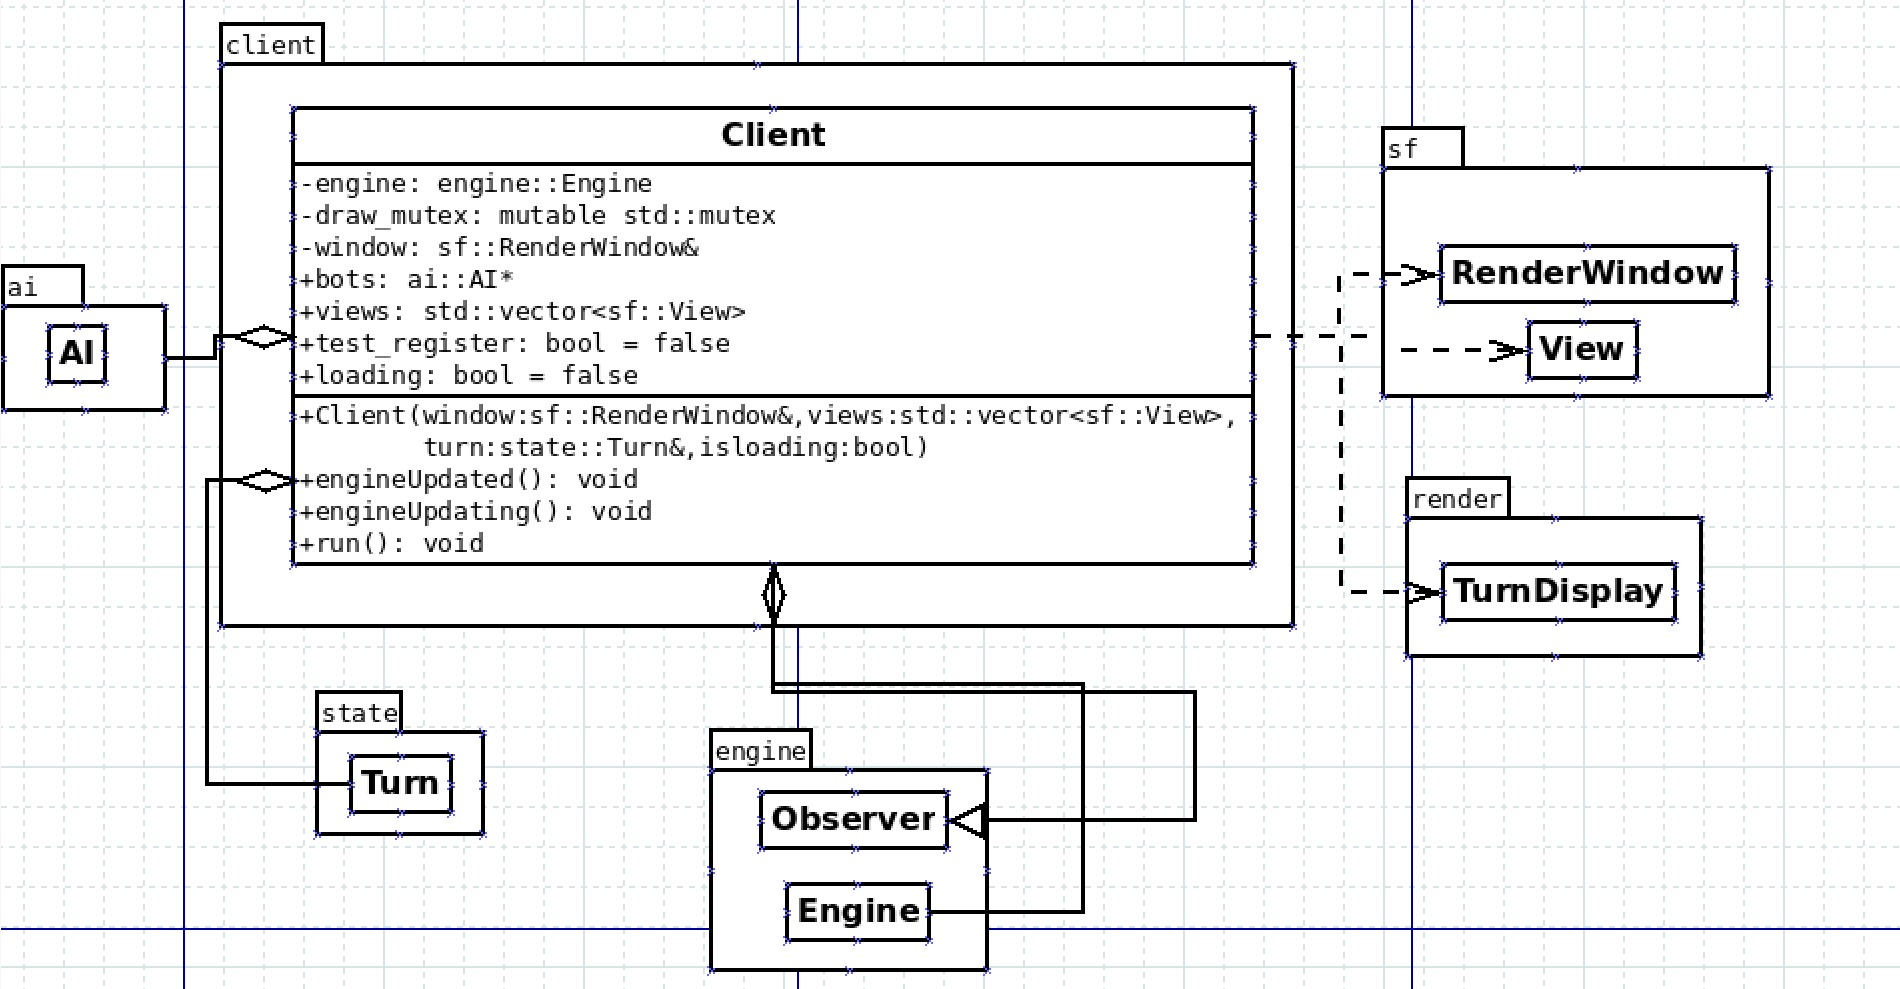
\includegraphics[width=\linewidth]{images/client_dia.png}
\centering
\caption{Aperçu de client.dia}
\label{fig:img6}
\end{figure}
\newpage
